\documentclass[tikz, border=10pt]{standalone}
\usepackage{tikz}
\usepackage{amsmath}
\usepackage{xcolor}
\usetikzlibrary{arrows.meta, positioning, calc, decorations.markings}

\definecolor{sensorBlue}{HTML}{1565c0}
\definecolor{waveOrange}{HTML}{e65100}
\definecolor{dotRed}{HTML}{c62828}
\definecolor{panelBg}{HTML}{fafafa}

\begin{document}
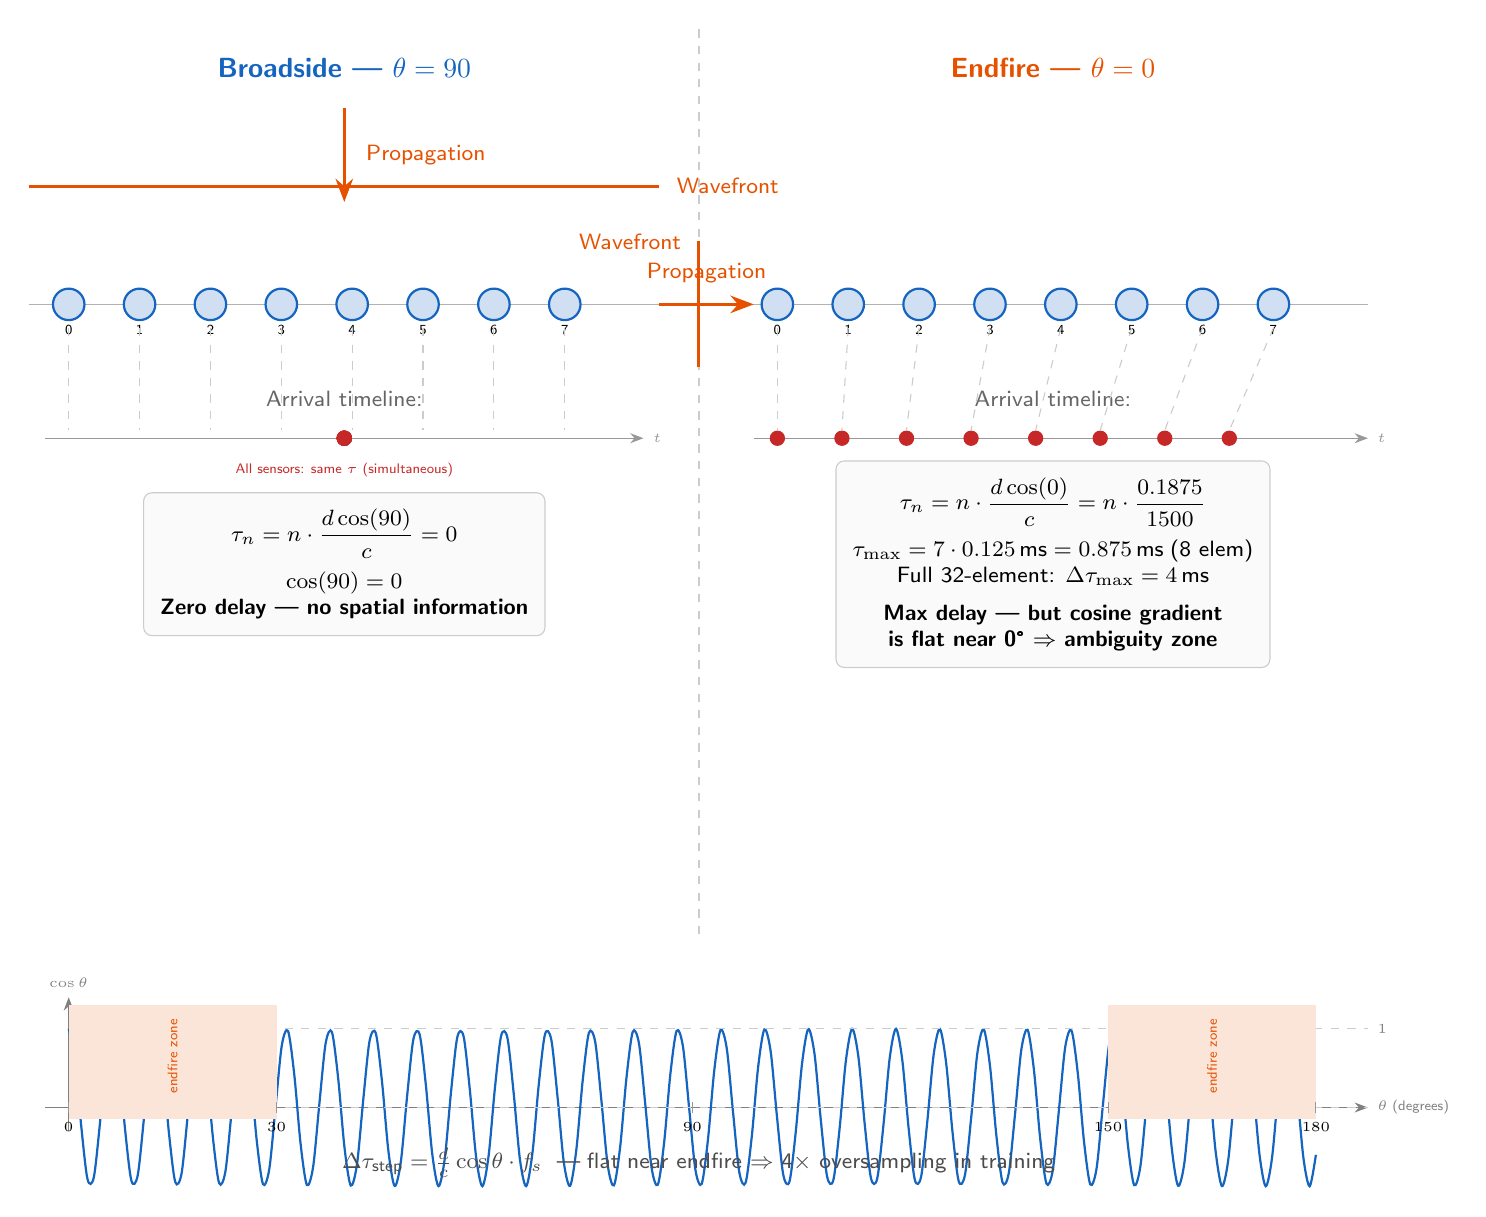
\begin{tikzpicture}[>=Stealth, font=\sffamily\small]

%% ── DIVIDER ──────────────────────────────────────────────────────────────
\draw[black!20, dashed, thick] (8.0, -5.0) -- (8.0, 6.5);

%% ════════════════════════════════════════════════════════════════════
%%  LEFT PANEL — BROADSIDE (θ = 90°)
%% ════════════════════════════════════════════════════════════════════
\node[font=\sffamily\normalsize\bfseries, sensorBlue] at (3.5, 6.0)
    {Broadside — $\theta = 90°$};

% ULA
\draw[black!30] (-0.5, 3.0) -- (7.5, 3.0);
\foreach \i in {0,...,7}{
    \draw[sensorBlue, fill=sensorBlue!20, thick]
        ({0.9*\i}, 3.0) circle (0.20);
    \node[below=4pt, font=\sffamily\tiny] at ({0.9*\i}, 3.0)
        {\i};
}

% Wavefront arrives from directly above (perpendicular to array)
% → horizontal line above the array
\draw[waveOrange, very thick, ->]
    (3.5, 5.5) -- (3.5, 4.3)
    node[midway, right=4pt, waveOrange, font=\sffamily\footnotesize]
    {Propagation};
\draw[waveOrange, very thick]
    (-0.5, 4.5) -- (7.5, 4.5);
\node[waveOrange, right, font=\sffamily\footnotesize] at (7.6, 4.5)
    {Wavefront};

% All arrivals simultaneous — timeline with all dots at same position
\node[font=\sffamily\footnotesize, black!60] at (3.5, 1.8)
    {Arrival timeline:};
\draw[->, thin, black!40] (-0.3, 1.3) -- (7.3, 1.3)
    node[right, font=\sffamily\tiny]{$t$};
\foreach \i in {0,...,7}{
    % All dots at the same x position → simultaneous arrival
    \filldraw[dotRed] (3.5, 1.3) circle (0.09);
    \draw[black!20, dashed, thin]
        ({0.9*\i}, 2.7) -- ({0.9*\i}, 1.4);
}
\node[font=\sffamily\tiny, dotRed] at (3.5, 0.9)
    {All sensors: same $\tau$ (simultaneous)};

% Annotation box
\node[draw=black!20, fill=panelBg, rounded corners=3pt,
      inner sep=6pt, font=\sffamily\footnotesize, align=center]
      at (3.5, -0.3) {
    $\tau_n = n\cdot\dfrac{d\cos(90°)}{c} = 0$\\[4pt]
    $\cos(90°) = 0$\\
    \textbf{Zero delay — no spatial information}
};

%% ════════════════════════════════════════════════════════════════════
%%  RIGHT PANEL — ENDFIRE (θ = 0°)
%% ════════════════════════════════════════════════════════════════════
\node[font=\sffamily\normalsize\bfseries, waveOrange] at (12.5, 6.0)
    {Endfire — $\theta = 0°$};

% ULA
\draw[black!30] (8.5, 3.0) -- (16.5, 3.0);
\foreach \i in {0,...,7}{
    \draw[sensorBlue, fill=sensorBlue!20, thick]
        ({9.0 + 0.9*\i}, 3.0) circle (0.20);
    \node[below=4pt, font=\sffamily\tiny] at ({9.0 + 0.9*\i}, 3.0)
        {\i};
}

% Wavefront arrives from the left (parallel to array axis)
% → vertical line to the left of element 0
\draw[waveOrange, very thick, ->]
    (7.5, 3.0) -- (8.7, 3.0)
    node[midway, above=4pt, waveOrange, font=\sffamily\footnotesize]
    {Propagation};
\draw[waveOrange, very thick]
    (8.0, 2.2) -- (8.0, 3.8);
\node[waveOrange, left, font=\sffamily\footnotesize] at (7.9, 3.8)
    {Wavefront};

% Progressive arrivals — dots shift to the right
\node[font=\sffamily\footnotesize, black!60] at (12.5, 1.8)
    {Arrival timeline:};
\draw[->, thin, black!40] (8.7, 1.3) -- (16.5, 1.3)
    node[right, font=\sffamily\tiny]{$t$};
\pgfmathsetmacro{\tscale}{0.82}
\foreach \i in {0,...,7}{
    \pgfmathsetmacro{\arrx}{9.0 + \i*\tscale}
    \filldraw[dotRed] (\arrx, 1.3) circle (0.09);
    \draw[black!20, dashed, thin]
        ({9.0 + 0.9*\i}, 2.7) -- (\arrx, 1.4);
}
\node[font=\sffamily\tiny, dotRed] at (12.5, 0.9)
    {Progressive: $\tau_n = n\cdot d/c = n \times 0.125\,\text{ms}$};

% Annotation box
\node[draw=black!20, fill=panelBg, rounded corners=3pt,
      inner sep=6pt, font=\sffamily\footnotesize, align=center]
      at (12.5, -0.3) {
    $\tau_n = n\cdot\dfrac{d\cos(0°)}{c}
             = n\cdot\dfrac{0.1875}{1500}$\\[4pt]
    $\tau_{\max} = 7\cdot0.125\,\text{ms} = 0.875\,\text{ms}$\;(8 elem)\\
    Full 32-element: $\Delta\tau_{\max} = 4\,\text{ms}$\\[4pt]
    \textbf{Max delay — but cosine gradient}\\
    \textbf{is flat near 0° $\Rightarrow$ ambiguity zone}
};

%% ── Cosine function sketch (bottom, full width) ──────────────────────────
\begin{scope}[yshift=-7.2cm]
\draw[->, thin, black!50] (-0.3, 0) -- (16.5, 0)
    node[right, font=\sffamily\tiny]{$\theta$ (degrees)};
\draw[->, thin, black!50] (0.0, -0.3) -- (0.0, 1.4)
    node[above, font=\sffamily\tiny]{$\cos\theta$};
\draw[sensorBlue, thick, smooth, domain=0:180, samples=200]
    plot ({0.088*\x}, {cos(deg(\x*1))});   % 0.088 maps 180deg to 15.8 units
\draw[black!20, dashed] (0, 1.0) -- (16.5, 1.0);
\node[right, font=\sffamily\tiny, black!50] at (16.5, 1.0) {$1$};
\draw[black!20, dashed] (0, 0.0) -- (16.5, 0.0);
% Endfire zones highlighted
\fill[waveOrange!15]
    (0, -0.15) rectangle ({0.088*30}, 1.3);
\fill[waveOrange!15]
    ({0.088*150}, -0.15) rectangle ({0.088*180}, 1.3);
\node[waveOrange, font=\sffamily\tiny, rotate=90]
    at ({0.088*15}, 0.65) {endfire zone};
\node[waveOrange, font=\sffamily\tiny, rotate=90]
    at ({0.088*165}, 0.65) {endfire zone};
% x-axis ticks
\foreach \deg/\lbl in {0/$0°$, 30/$30°$, 90/$90°$, 150/$150°$, 180/$180°$}{
    \draw[thin, black!40] ({0.088*\deg}, -0.07) -- ({0.088*\deg}, 0.07);
    \node[below, font=\sffamily\tiny] at ({0.088*\deg}, -0.07) {\lbl};
}
\node[font=\sffamily\footnotesize, black!70]
    at (8.0, -0.7)
    {$\Delta\tau_{\text{step}} = \tfrac{d}{c}\cos\theta \cdot f_s$
     \;---\;flat near endfire $\Rightarrow$ 4$\times$ oversampling in training};
\end{scope}

\end{tikzpicture}
\end{document}
